% This is samplepaper.tex, a sample chapter demonstrating the
% LLNCS macro package for Springer Computer Science proceedings;
% Version 2.20 of 2017/10/04
%
\documentclass[runningheads]{llncs}
\usepackage{amsmath}
\usepackage{hyperref}
%
\usepackage{graphicx}
% Used for displaying a sample figure. If possible, figure files should
% be included in EPS format.
%
% If you use the hyperref package, please uncomment the following line
% to display URLs in blue roman font according to Springer's eBook style:
% \renewcommand\UrlFont{\color{blue}\rmfamily}

\begin{document}
%
\title{Distributed Teams Are Founded on Explicit
Communication Channels}
%
%\titlerunning{Abbreviated paper title}
% If the paper title is too long for the running head, you can set
% an abbreviated paper title here
%
\author{Het Jatin Dalal}
%

%
\institute{Computer Science and Software Engineering , Concordia University \\ 
\vspace{10pt}  VCS: Github: \href{https://github.com/Het95/40200513-SOEN6481-TAS}{https://github.com/Het95/40200513-SOEN6481-TAS}}

%
%
\maketitle              % typeset the header of the contribution
%

\begin{abstract}
    The abstract should briefly summarize the contents of the paper in
    15--250 words.
    
    \keywords{First keyword  \and Second keyword \and Another keyword.}
    \end{abstract}
    %
    %
    %
    \section{Introduction}
    \subsection{Motivation}

    \begin{figure}   
        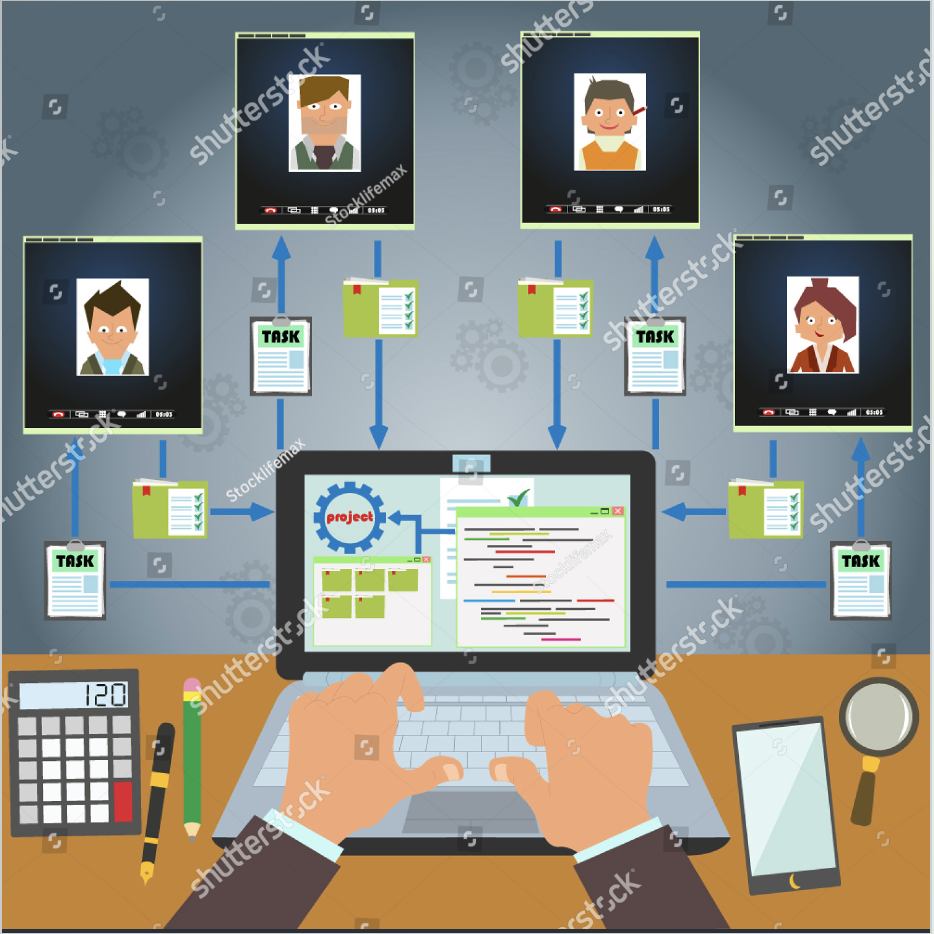
\includegraphics[width=0.2\linewidth]{DTlogo.png}
    \end{figure}

    The motivation for researching "Distributed Teams Established on Explicit Defined Communication Channels" stems from a number of key considerations and the difficulties of modern work contexts.
    
    \begin{enumerate}
        \item \textbf{Surge in popularity of Distributed Team}: The majority of businesses with growing workforces are shifting to distributed team structure, particularly in light of recent pandemics like COVID-19. This makes it much more important in such an environment to collaborate and communicate effectively.. 
        \item \textbf{Accountability}: Having clear channels of communication within the team facilitates awareness of individual roles and responsibilities.
        \item \textbf{Collaboration}: Distributed teams can share project-related materials and do various other project management tasks with each other when they have clear communication channels. 
        \item \textbf{Embrace, Evolve, Adjust}: One must adjust to the changing environment due to changes in new technology, team and company sizes, and the organization can concentrate more on this by employing clear communication channels.
    \end{enumerate}
    
    \subsection{Problem Statement} In distributed team environment, the challenge of effective in-person communication has emerged due to its larger size. Interruptions for resource retrieval are also causing productivity loss, especially when team members are intently focused. The necessity for well-defined communication channels has evolved, accompanied by disputes over the advantages of synchronous versus asynchronous systems. There is a need to build a culture of written communication and to decisively identify and implement clear and effective communication channels in distributed team environment in order to unlock quick growth and better productivity.~\cite{refbook1}

    \subsection{Objectives} In this investigation, the key objective of the analysis is to describe the significance of using clear and explicit communication channels within distant work environments to boost productivity, efficiency, reducing interruptions, fill information gaps while also allowing them to grow faster. The ultimate objective is to elevate team performance to a new level, promote alignment, preparing teams to work remotely and build resilient teams that can adjust to change.This will help to simplify project management, particularly when adding new team members, and will be advantageous to managers, team leaders, and team members alike. ~\cite{refbook1}

    \section{Background Material}
For the context of the report, it is important to know all the following terms in order to gain proper understanding.

 \begin{itemize}
    \item \textbf{Distributed/Remote Teams}: The Distributed Team is spread over the same rooms, city, and possibly even continent. In a nutshell, it consists of two or more people who do not share the same physical workspace or geographical location.~\cite{refbook1}\\
    \item \textbf{Communication Challenges}: Team members' productivity may suffer if they are unclear about where to obtain information or how to communicate well. They could squander time attempting to find information or cause their teammates needless disruptions. causing tap on the shoulder or chat app notifications, when working in deep focus mode ~\cite{refbook1}\\
    \item \textbf{Synchronous and Asynchronous communication channels}: 
    Synchronous communication channels, which primarily include voice messages, video conferencing apps, instant messaging apps, and in-person meetings if dispersed nearby, can be used to facilitate real-time dialogue between various team members from all walks of life, from information technology to hospitals~\cite{refbook1}~\cite{refpaper1}.
    Asynchronous communication channels , which primarily include collaborative documents like Google Docs, forums, task tracking applications like Jira, Trello, and emails~\cite{refarticle1}, can be used to avoid real-time talk and communicate as needed or by deadline.~\cite{refbook1}
\end{itemize}


    \begin{thebibliography}{8}
        \bibitem{refbook1}
        97 Things Every Engineering Manager Should Know [Book],” www.oreilly.com. \url{https://www.oreilly.com/library/view/97-things-every/9781492050896/}
        \bibitem{refpaper1}
        E. Coiera, “Communication systems in healthcare,” The Clinical biochemist. Reviews, vol. 27, no. 2, pp. 89–98, 2006, \url{https://www.ncbi.nlm.nih.gov/pmc/articles/PMC1579411/} 
        \bibitem{refarticle1}
        What is Asynchronous Communication and How Do Teams Use It?,”\url{https://www.betterup.com/blog/asynchronous-communication}
    \end{thebibliography}
    
\end{document}
